% ----------------------------------------------- 
%  Plantilla LaTeX para el Trabajo Fin de Grado
%         Facultad de Ciencias
%        Universidad de Córdoba
%             Codificación utf8
%------------------------------------------------
%              Abril 2022
%------------------------------------------------
\documentclass[12pt,a4paper]{report}

% Fichero de estilo proporcionado
%%%%%%%%%%%%%%%%%%%%%%%%%%%%%%%%%%%%%%%%%%%%%%%%%%%%
%%
%% Este es el fichero 'estilo_TFG_CienciasUCO_2022.sty'
%%    con el estilo LaTeX para escribir los
%%          TRABAJOS FIN DE GRADO
%%                 de la 
%%          Facultad de Ciencias 
%%         Universidad de Córdoba
%               Abril 2022
%    
%           CODIFICAIÓN utf-8
%%%%%%%%%%%%%%%%%%%%%%%%%%%%%%%%%%%%%%%%%%%%%%%%%%%%%



% Idioma castellano 
\usepackage[utf8]{inputenc}
\usepackage[T1]{fontenc}
\usepackage[english]{babel}
%\usepackage{mathpazo} 
%\usepackage{eulervm}


% Tamaño de la página
\usepackage[left=2.5cm,right=2.5cm,top=2cm,bottom=2cm]{geometry}
\renewcommand{\pagename}{Page}

% Para redefinir algunas cosas del babel en castellano 
%\accentedoperators    % Pone acentos a los operadores
%\decimalpoint         % Usa el punto como separador decimal
                    

% Paquetes auxiliares  (incluir aquellos que se necesiten)

\usepackage[usenames,dvipsnames]{xcolor} % Para usar colores
\usepackage{tikz}                        % Para dibujar
\usepackage[strict]{changepage}          % Para redefinir márgenes en mitad del documento

% Para matemáticas
\usepackage{amsmath}
\usepackage{amsfonts}
\usepackage{amssymb}

% Para gráficos
\usepackage{graphicx}
\usepackage{subfigure}
\usepackage{float}
%
\usepackage{appendix}   % Contiene mandatos adicionales para apéndices
\usepackage{titlesec}   % Para redefinir capítulos, secciones,...
\usepackage{longtable}  % Para tablas grandes


% Para las cabeceras y pies (luego se redefine cuando haga falta)
\usepackage{fancyhdr}   % Para las cabeceras
\pagestyle{fancy} 
\fancyhf{}
\renewcommand{\headrulewidth}{0pt}
\renewcommand{\footrulewidth}{0pt}

%Para el fondo de la portada
\usepackage{eso-pic}
\newcommand\BackgroundPic{%
\put(0,0){%
\parbox[b][\paperheight]{\paperwidth}{%
\vfill
\centering

\includegraphics[width=\paperwidth,height=\paperheight,%
keepaspectratio]{fondo_portada.png}%
\vfill
}}}

% Estilo de capítulo, secciones...

\titlespacing*{\chapter}{0pt}{50pt}{40pt}
\titleformat{\chapter}[display]
  { \sffamily\bfseries\Large\color{blue}}
  {\filleft\MakeUppercase{\chaptertitlename}\ \Huge\sffamily{\arabic{chapter}}\ 
  }  
  {4ex}
  {\titlerule
   \vspace{2ex}%
   \filright}
  [\vspace{2ex}\hrule\vspace{2pt}%
   \titlerule]
   
   \titleformat{\section}[hang]
{\large \scshape\bfseries}
{\color{blue}  \thesection .}
{1ex}{\color{blue}}[\quad]
{}

  \titleformat{\subsection}[runin]
{ \scshape\bfseries}
{\color{blue}  \thesubsection .}
{1ex}{\color{blue}}[\quad]
{}
   
%%%%%%%%%%%%%%%%%%%%%%%%%%%%%%%%%%%%
% Para los códigos 
\usepackage{listings}

% Para código Matlab
\lstset{language=Matlab,
  keywords={break,case,catch,continue,else,elseif,end,for,function,
      global,if,otherwise,persistent,return,switch,try,while,diary,
      clear,clc,who,whos,help,helpwin,linspace,length,ans,doc,floor,
      ceil,max,min,sum,prod,sort,round,sign,fix,mean,exp,sin,cos,tan,
      input,fprint,load,save,disp,fopen,fclose,inline,function,feval,
      global,return,poly,polyval,roots,solve,fzero, poly2sym,hold,plot,
      polyfit,ppval,spline,interp1,quad,quadl,quadgk,inv,\,lu,cond,spdisgs,
      magic,ode*,ode45,ode23,flops,rref,pinv,chol,zeros,ones,rand,sparse,
      tic,toc,diag,eye,speye,espones,spy,syms,diff,dsolve,simplify,ezplot},
   basicstyle=\small \ttfamily,
   keywordstyle=\color{blue},
   commentstyle=\color{webgreen},
   stringstyle=\color{webtinto},
   numbers=left,
   numberstyle=\tiny\color{gray},
   stepnumber=1,
   numbersep=10pt,
   backgroundcolor=\color{white},
   tabsize=4,
   showspaces=false,
   showstringspaces=false,
%
   frame=LtbR,
     framerule=0.5pt,
     aboveskip=0.5cm,
     framextopmargin=3pt,
     framexbottommargin=3pt,
%     framexleftmargin=1cm,
     framesep=0pt,
     rulesep=.4pt,
     backgroundcolor=\color{gray96},
     rulesepcolor=\color{black}}
     
     
 % Para código ISE
     
\lstdefinelanguage{ISE} {morekeywords={library,use,entity,is,port,in,out,end,
               architecture,of,is,signal,begin,process,then,
               port,downto,if,and,then,else
               },                
sensitive=false,
emph={STD_LOGIC_1164,
STD_LOGIC_ARITH,
STD_LOGIC_UNSIGNED,
IEEE,
ALL,
STD_LOGIC,
STD_LOGIC_VECTOR}, 
emphstyle=\color{magenta},
morecomment=[l]{--},
basicstyle=\small \ttfamily,
   keywordstyle=\color{blue},
   commentstyle=\color{webgreen},
   stringstyle=\color{webtinto},
   numbers=left,
   numberstyle=\tiny\color{gray},
   stepnumber=1,
   numbersep=10pt,
   backgroundcolor=\color{white},
   tabsize=4,
   showspaces=false,
   showstringspaces=false,
%
   frame=LtbR,
     framerule=0.5pt,
     aboveskip=0.5cm,
     framextopmargin=3pt,
     framexbottommargin=3pt,
%     framexleftmargin=1cm,
     framesep=0pt,
     rulesep=.4pt,
     backgroundcolor=\color{gray96},
     rulesepcolor=\color{black}
     }
     
%para generar índice con hipervínculos
\usepackage{hyperref} 



\hypersetup{
    colorlinks,
    citecolor=webgreen,
    filecolor=black,
    linkcolor=webblue,
    urlcolor=webtinto,
}


% Colores definidos
\definecolor{azul}{rgb}{65,105,225}
\definecolor{webgreen}{rgb}{0,.5,0}
\definecolor{webgray}{rgb}{.753,.753,.753}
\definecolor{webblue}{rgb}{0,0,.8}
\definecolor{webtinto}{rgb}{0.73,0.00,0.00}
\definecolor{gray96}{gray}{.96}

% Algunas redefiniciones 
%\renewcommand{\contentsname}{Índice general}
%\renewcommand{\partname}{Parte}
%\renewcommand{\appendixname}{Apéndice}
%\renewcommand{\figurename}{Figura}
%\renewcommand{\listfigurename}{Índice de figuras}
\renewcommand{\chaptername}{Chapter}
%\renewcommand{\bibname}{Bibliografía}




%%%% Nuevas definiciones %%%%%%%%%%%%%%%%%%%%%%%%%%%%%%%

% Ejemplos de algunas definiciones 
\def \dint{\displaystyle \int}
\def \gt {\gamma(t)}        %  gamma(t)
\def \st {\tilde{\sigma}}   %  sigma tilde
\def \sg {\sigma_{\gamma}}  %  sigma sub gamma
\def \omt {\omega(t)}       %  omega(t)
\def \bu {\mathbf{u}}       %  u negrilla
\def \R {\mathbb{R}}        %  números reales
\usepackage{siunitx}


%--------------------------------------------------------------------------------------
% CAMBIAR LOS DATOS EN CADA CASO 

\newcommand{\titulacion}{Grado de Física}                  % Grado de Biología
                                                      % Grado de Bioquímica
                                                      % Grado de Ciencias Ambientales
                                                      % Grado de Física
                                                      % Grado de Química
                                                      
\newcommand{\titulo}{Oscilaciones Bariónicas Acústicas en Universos con Curvatura} % Título
\newcommand{\codigo}{FS22-17-FSC}      % Código
\newcommand{\tipo}{Trabajo teórico-práctico general}             % Trabajo teórico--práctico general
                                          		     % Trabajo de iniciación a la investigación
                                                      % Trabajo en empresa
                                                      % Idea de negocio
                                                      % Propuesta científico--técnica
                                                      % Trabajo docente
                                          
\newcommand{\autor}{Santiago Sanz Wuhl}     % Autor
\newcommand{\fecha}{Fecha de entrega}                 % Fecha de entrega
%--------------------------------------------------------------------------------------
\newcommand{\nomfig}{Figura}                         
\newcommand{\nomfigs}{figures} 

% Si se quiere que las figuras se denominen ilustraciones comentar las dos órdenes
% anteriores y descomentar las dos que siguen 

%\newcommand{\nomfig}{Ilustración}                         
%\newcommand{\nomfigs}{ilustraciones}   


%--------------------------------------------------------------------------------------

% Empieza el documento
\begin{document}

% No cambiar  %%%%%%%%%%%%%%%%%%%%%%%%%%%%%%%%%%%%%%%%%%%%%%%%%%%%%%%%%%%%
%%%%%%%%%%    NO CAMBIAR   %%%%%%%%%%%%%%%%%%%%%%%%%%%%%
% Inclusión automática de la portada, tribunal e índices
%%%%%%%%%%    NO CAMBIAR   %%%%%%%%%%%%%%%%%%%%%%%%%%%%%%

% PORTADA----------------------------------
\AddToShipoutPicture*{\BackgroundPic}
\begin{titlepage}
\begin{center}
\Large UNIVERSIDAD DE CÓRDOBA\\[0.5 cm]
\large  \textbf{Facultad de Ciencias}\\[1.25 cm]
\large \textbf{\titulacion}\\[1.25 cm]
\Large  Trabajo Fin de Grado\\[2.25 cm]
\Huge   \titulo
\end{center}
\vspace{1.25cm}
\noindent {\large Código del TFG: \textbf{\color{blue}\codigo}}\\[0.3cm]
\noindent {\large Tipo de TFG: \textbf{\color{blue}\tipo}}\\[0.5cm]
{\color{blue}\hrule}
\vspace{0.5cm}
\noindent \Large{Autor: \autor}
\vfill
\begin{center}
 
\includegraphics[width=6cm]{logo_ciencias.png} 
\end{center}
\vfill
\rightline{\fecha}
\end{titlepage}
\renewcommand{\baselinestretch}{0.9}
\ClearShipoutPicture

 %%%%%%%%%%%%%%%%%%%%%%%%%%%%%%%%%%%%%%%%%%%%%%%%%%%%%%%%%%%%%%%%%%




   % Dejar esta línea (incluirá el fichero 		 
%                                  portada.tex
% 	                              proporcionado, que no hay que modificar
% Fin de No cambiar %%%%%%%%%%%%%%%%%%%%%%%%%%%%%%%%%%%%%%%%%%%%%%%%%%%%%%%


\fancypagestyle{plain}{
\fancyfoot[R]{\large{pág. \thepage}}
}

\pagestyle{fancy} 

\chapter*{Agradecimientos}

Agradecer antes que nada a mi familia; mi padre Fernando, mi madre Judith y mi hermana Sofi por apoyarme y lo que es más importante, soportarme todos estos años. Fuisteis el apoyo sin el cual no podría haber llegado hasta donde he llegado.

Por otro lado, a todos/as aquellos profesores que me motivaron a tomarme en serio esta carrera y seguir en el camino de la investigación, entre los cuales se encuentra y con razón, mi tutor Antonio J. Cuesta. Dentro del departamento, agradecer también al profesor Alberto Jiménez del Dpto. de Física de la Universidad de Córdoba el facilitarme el acceso a los ordenadores del grupo \textit{FQM-378}.

Finalmente, agradecer a todas las personas que están detrás de este trabajo, desde la Universidad de Córdoba; Antonio J. Cuesta, Antonio Sarsa, y desde la Universidad de Barcelona, Héctor Gil-Marín y Licia Verde por ofrecer los códigos de análisis BRASS y RUSTICO utilizados en este trabajo de Fin de Grado.
 % Agradecimientos y/o dedicatoria si procede (si no comentar esta línea)

% No cambiar  %%%%%%%%%%%%%%%%%%%%%%%%%%%%%%%%%%%%%%%%%%%%%%%%%%%%%%%%%%%%
% INDICES-----------------------------------

% Genera el índice de contenidos------------

\fancypagestyle{plain}{
\fancyfoot[R]{\small pág. \thepage} 
}
\tableofcontents
\addcontentsline{toc}{chapter}{Índice general}

\renewcommand{\baselinestretch}{1.5}

% Genera el índice de figuras---------------
\fancypagestyle{plain}{
\fancyfoot[R]{\small pág. \thepage} 
}
\renewcommand{\listfigurename}{Índice de \nomfigs}
\renewcommand{\figurename}{\nomfig}

\listoffigures
\addcontentsline{toc}{chapter}{Índice de \nomfigs}


% Genera el índice de tablas---------------
\fancypagestyle{plain}{
\fancyfoot[R]{\small pág. \thepage}
}
\listoftables
\addcontentsline{toc}{chapter}{Índice de tablas}


% Para las cabeceras del resto

\pagestyle{fancy} 
\fancyhf{}
\fancyfoot[R]{\small pág. \thepage}
\renewcommand{\headrulewidth}{0pt}
\renewcommand{\footrulewidth}{0pt}  % Dejar esta línea (incluirá el fichero 		 
%                                  indices.tex
% 	                              proporcionado, que no hay que modificar
% Fin de No cambiar %%%%%%%%%%%%%%%%%%%%%%%%%%%%%%%%%%%%%%%%%%%%%%%%%%%%%%%


\chapter*{Resumen}
\addcontentsline{toc}{chapter}{Resumen. Palabras clave}

En este trabajo de fin de grado se hace uso de herramientas de computación de alto rendimiento y análisis de datos para estudiar los efectos de ligeras variaciones en el modelo cosmológico estándar, el modelo $\Lambda$ \textit{Cold Dark Matter} ($\Lambda$CDM). Si bien este modelo asume un universo espacialmente plano, se observa que las variaciones de hasta un 20\% en el parámetro de curvatura del universo $\Omega_k$ no tienen consecuencias significativas en los observables que nos interesan.

Este trabajo se basa en las oscilaciones acústicas de bariones, un fenómeno que nos permite estudiar el comportamiento del universo en sus etapas más tempranas (los primeros 380.000 años de sus 13.800 millones de años de vida, ¡un 0,03\% de la vida del universo!). Estas oscilaciones dan forma a la estructura a gran escala del universo y, lo que es más importante, establecen una "regla cósmica" $r_d$ con respecto a la cual se miden las distancias cosmológicas, como la distancia de Hubble $D_H$ y la distancia del diámetro angular $D_M$.

Después de analizar el catálogo de galaxias de la encuesta espectroscópica de oscilaciones acústicas de bariones extendida, se obtuvieron los siguientes resultados: $D_H/r_d = 18.66\pm 0.72$ y $D_M/r_d = 18.28\pm 0.53$ para un universo plano, en concordancia con los resultados para todos los valores del parámetro $\Omega_k$ indicados, y lo que es más importante, con resultados anteriores en el campo.

\paragraph{Palabras clave:} Cosmología; Astrofísica; Oscilaciones Acústicas de Bariones; Análisis de datos.









\chapter*{Abstract}
\addcontentsline{toc}{chapter}{Abstract. Keywords}

In this Bachelor's Thesis we make use of high performance computing and data analysis tools to study the effects of slight variations in the Standard Cosmological model, the $\Lambda$ Cold Dark Matter ($\Lambda$CDM) model. While this model assumes a spatially flat universe, we observe that variations of around 20\% in the curvature parameter of the universe $\Omega_k$ have no significant consequences in the observables that interest us.\\

This work is based off the Baryon Acoustic Oscillations, a phenomenon that allows us to study the behaviour of the universe in its earliest stages (the first 380.000 of its 13.8 billion years of lifetime -- a 0.03\% of the Universe's lifetime!). These oscillations shape the large scale structure of the universe, and more importantly, set a `cosmic ruler' $r_d$ with respect to which is used to measure cosmological distances, such as the Hubble distance $D_H$ and angular diameter distance $D_M$.\\

After analyzing the extended Baryon Oscillation Spectroscopic Survey galaxy catalogue, we achieve the following results: $D_H/r_d = 18.66\pm 0.72$ y $D_M/r_d = 18.28\pm 0.53$ for a flat universe, in concordance to the results for all the stated  $\Omega_k$ parameter values, and more importantly with previous results in the field.





\paragraph{Keywords:} Cosmology; Astrophysics; Baryon Acoustic Oscillations; Data Analysis.
          % Resumen (insertar en el fichero resumen.tex proporcionado,
%                                     el resumen en español e inglés)

% empiezan los capítulos
\chapter{Introduction}

\section{The Hot Big Bang model}

The most accepted model for the origin of the universe is the Big Bang model, that models the beginning of the universe as a hot dense state. The Big Bang surprisingly to some conveys no "bang", but the sudden existence of all the matter in the universe, in the shortest of times, in the smallest of spaces, about 13.8 billion years ago. After an unthinkably small interval of time, the universe began a short period of rapid expansion known as \textit{cosmic inflation}, in which the universe grew by a factor $10^{27}$ in a mere $10^{-33}$ seconds. This inflation is thought to be due to the inflaton, a quantum scalar field. It is theorized that it is the inflaton's vaccuum energy what caused the universe to expand as greatly. \\

As any quantum field\footnote{Quantum fields are a tool used by Quantum Field Theory (QFT) to more accurately describe particles and their interactions, at high enough energies.} the inflaton presents fluctuations. This means, even in the vacuum state\footnote{To define vacuum in QFT is not as easy a task as it was in classical mechanics (or even non-relativistic quantum mechanics).These details go beyond the scope of this paper, and thus will not be dealt with.} there is constant creation and annihilation of particles. These fluctuations are what cause anisotropies in the matter distribution of the universe, fact that will be important later in this work. \\

After the inflation phase, the universe cooled enough for what is known as the Quark-Gluon plasma to form. In this state, temperatures were high enough as to consider relativistic the random motion of the particles in it. After some cooling due to cosmic expansion, the combination between quarks to form hadrons was allowed, leading to what is known as the hadronic epoch. However, due to the short mean free path of the photons, the universe is still opaque to electromagnetic radiation. \\

As the universe kept expanding the densities decreased and the temperatures cooled, the existence of atoms was starting to be allowed, the $He$ and $H$ atoms. This period would finish at the universe age of $380,000$ years, moment known as recombination. Recombination is thought of as the time at which the Thomson Scattering mechanisms stop being effective (the scattering cross section of this process becomes negligible and thus the photon mean free path grows considerably).
As soon as recombination ends, the thermally activated photons which are no longer energetic enough to interact with the electrons now travel freely through space. This emission is known as the Cosmic Microwave Background (CMB) and is the oldest direct observation using electromagnetic radiation we can take of the universe. \\

Though the name `recombination' implies the fact that the universe used to be `combined' and then ceased to be so, it just comes from the fact that recombination was theorized before the Big Bang theory was thought of. \\



\begin{figure}[t]
	\centering
	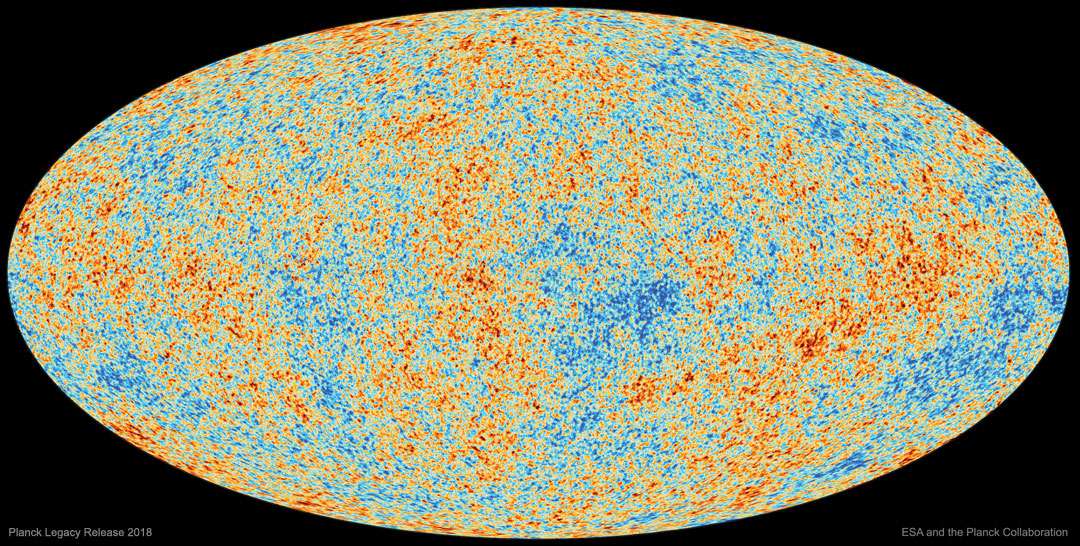
\includegraphics[width=0.8\textwidth]{../figs/cmb.jpeg}
	\caption[The all-sky map of CMB anisotropies as seen by space-based Observatory Planck]{The all-sky map of CMB anisotropies as seen by Space-based Observatory Planck \cite{Planck2018}. The colors in this map represent the fluctuations of the mean T = \SI{2.7}{K} with fluctuations of $10^{-5}$ with respect to the average temperature. Red means higher temperature than the average, whilst blue means lower temperature than the average.}
	\label{fig:cmb}
\end{figure}
\section{Cosmic Microwave Background}

We see in the figure~\ref{fig:cmb} the CMB as observed by the Planck colaboration \cite{Planck2018}. The radiaton we observe is the photons that were emmitted about $13.8$ billion years ago. Since the CMB appears as a result of the thermal photons emitted by the electrons in the primordial plasma, it offers great insight into what the plasma looked like, and the way it behaved.  \\

The Cosmic Microwave Background was discovered in 1965 as a serendipity by Penzias and Wilson \cite{Penzias1965}. They observed a noise signal, uniformly distributed\footnote{It was not actually uniformly distributed, since there was a small doppler shift due to the Earth's relative movement to the CMB. Surprisingly, even after removing this and other similar effects, it still presents minute fluctuations. These fluctuations, as it will be seen in the next sections contain a great deal of information on the composition of the universe and explains the origin of structure formation.} from every direction, day or night, summer or winter, almost as if it came directly from the origin of the universe.
This discovery was considered to be solid evidence for the Big Bang model and more importantly, the beginning of the modern cosmology. All of this became the reason Penzias and Wilson received a Nobel prize 13 years later, in 1978. \\

Since what is being measured are the photons left from recombination, which corresponds to a thermal radiation curve, we may use Wien's displacement law  \\
\begin{align}
	T = \frac{b}{\lambda}
	\label{eq:wien-displacement}
\end{align}
with $b\approx $ \SI{2.897}{mmK} Wien's constant, $T$ the black body radiation and $\lambda$ the wavelength at which the spectral radiation intensity is maximum to calculate the corresponding temperature to the measured wavelength. Using Planck's law, the measured temperature is \SI{2.7}{K} which corresponds to a measured wavelength of \SI{1.06}{mm} (microwave radiation, as the name Cosmic \textit{Microwave} implies). \\

In 1991 anisotropies in the CMB were first discovered, by the COBE satellite\cite{SmootMather} later earning Smoot and Mather a nobel prize. As of 2023 the most precise measurements correspond to the Planck experiment in 2018 \cite{Planck2018} by the European Space Agency. These anisotropies can be seen in \ref{fig:cmb}. \\

Of course, \SI{2.7}{K} was not the temperature of the plasma at recombination, as it was approximately hotter by a factor $z=1090$, or $\approx$\SI{3000}{K}. The reason we measure such smaller temperatures is because of the expansion of the universe. \\
If today ($t=t_0$) some radiation of wavelength $\lambda_o$ is observed, that somehow is known to have been travelling for some time $\Delta t$ will have stretched due to the expansion of the universe. In other words, the wavelength $\lambda_e$ of the emitted radiation was smaller by a factor\footnote{The factor $a(t)$ is known as the scale factor of the universe, and will be explained with further detail later in the work.} $a(t')^{-1}$, with $t' = t_0-\Delta t$ being the earlier time at which the radiation was emitted, and $a(t_0)=1$ by definition. By Wien's displacement law \eqref{eq:wien-displacement}, this corresponds to a higher temperature by a factor $a(t')$. \\


Thus, the CMB becomes crucial in explaining the large scale structure of the universe, since the photons that decoupled from the plasma at recombination wasted more energy leaving denser regions behind losing thermal energy in the process. Appearing at a slightly lower temperature (gravitational redshift). On the contrary, those in void regions will appear hotter, being blueshifted. Therefore, temperature fluctiations in the CMB correspond to density fluctuations in the early universe. \\

\section{Baryon Acoustic Oscillations}

\begin{figure}[t]
	\centering
	\subfigure[Origin of the BAO]{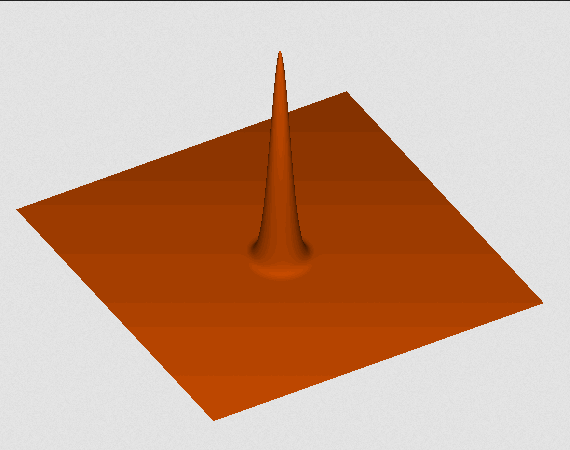
\includegraphics[width=0.3\textwidth]{baogif1.png}}
	\subfigure[The BAO propagating through the plasma]{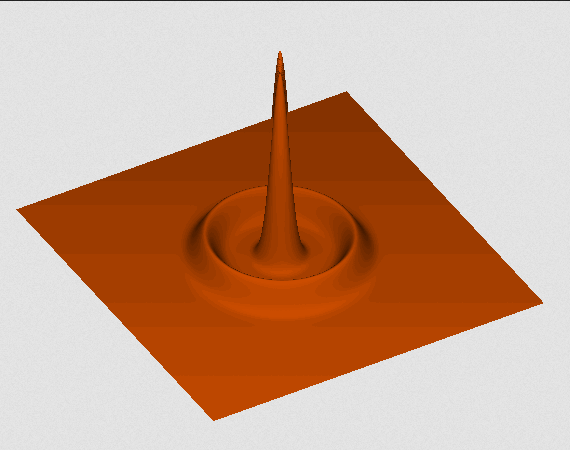
\includegraphics[width=0.3\textwidth]{baogif2.png}}
	\subfigure[The frozen BAO after recombination]{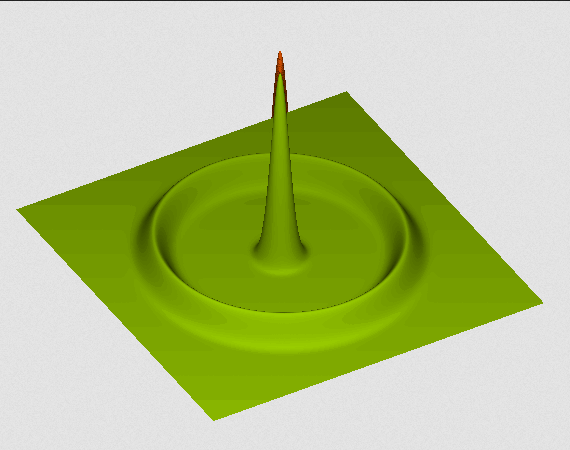
\includegraphics[width=0.3\textwidth]{baogif3.png}}
	\caption[Different stages of the Baryon Acoustic Oscillations.]{Different stages of the Baryon Acoustic Oscillations. Courtesy of the image (cite https://lweb.cfa.harvard.edu/~deisenst/acousticpeak/anim.gif)}
\end{figure}

Before recombination, both matter and photons were coupled into the same fluid which we have called the primordial plasma. The particles in the plasma interacted primarily with one another through gravity and electromagnetism, depending on the type of matter considered.  \\

As already mentioned, matter was not distributed homogenously. At some point in time before recombination one could find `lumps' of dark and baryonic (standard) matter. Combining the restoring force of the gravitational attraction between dark and baryonic matter with itself and with one another, and the repulsion caused by the radiation pressure due to the Thomson Effect between baryons and photons, the results are pure acoustic waves propagating through the plasma, with the dark matter lumps being in the center of these waves. Since the baryonic matter is dragged by these sound waves, they are called Baryon Acoustic Oscillations (BAO). \\


The waves would propagate throughout the plasma as long as the baryon-photon interaction was strong enough i.e. up to recombination, at which point they froze in time leaving higher density regions. Higher density means higher gravitational intensity, which in turn means higher galaxy proliferation in spherical distributions. These spherical distributions (which can be measured in the CMB) are what is known as the large scale structure of the universe. \\

At big enough distances, the radii ($r_s$) of these spheres, also called the sound horizon is used as a `cosmic ruler'. Big scale measurements are calculated in terms of $r_s$, which is measured from the CMB. This means it needs to be calibrated from external information. $ r_s$ has been measured from the CMB to be around  \SI{150}{Mpc} or 500 million lightyears.
To give an idea of the size of $r_s$, the radius of the observable universe is around 100 times $r_s$. \\

Given the large dimensions of this cosmic ruler and the homogeneity of the universe on large scales, this ruler is only affected by cosmological expansion rather than late-time gravitational effects. Therefore, it has a constant comoving\footnote{`Comoving' meaning the distance one would measure had the expansion of the universe not existed} size throughout the universe.

These structures were observed for the first time in 2005 simultaneously both by the 2dF Galaxy Redshift Survey\cite{2dFCole2005} and the Sloan Digital Sky Survey\cite{Eisenstein2005}, the results of which can be seen in the figure \ref{fig:2005-results}. In these pictures one sees the correlation function  $\xi(r)$ and the power spectrum $P(k)$ (though in the figure \ref{fig:2df} it is called $W_k$). These are the main tools for the study of the BAO.
The correlation function $\xi(s)$, with $s$ being a distance variable measures the frequency of the separation between any two galaxies. If the BAO hypothesis is true, then one would find a local maximum at $r_s$, the radius of the frozen spherical waves. \\

The other tool for studying the BAO is the power spectrum seen in \ref{fig:2df}. It is, without need of more detail, the Fourier transform of the $\xi(s)$ function. Indeed, since there is a repeating pattern of wavelength $r_s$, one would find local maxima in the spectrum at integer multiples of $k = 2\pi /r_s$. \\

\begin{figure}[t] \centering
	\subfigure[The correlation function $\xi(s)$ as measured by the Sloan Digital Sky Survey \cite{Eisenstein2005}]{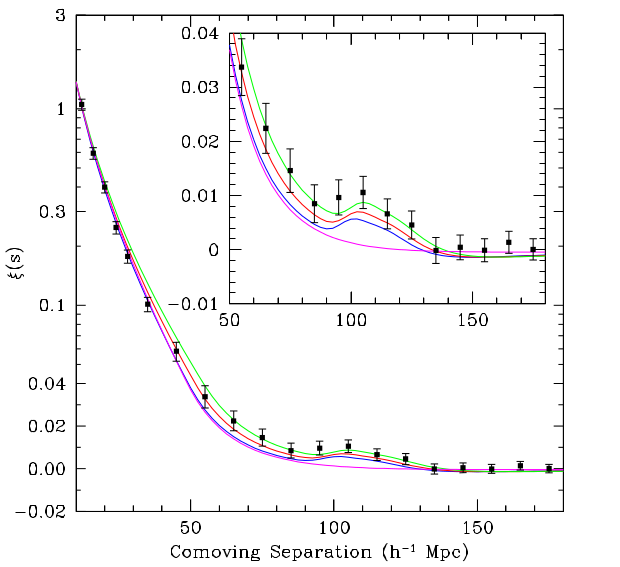
\includegraphics[width=0.4\textwidth]{../figs/sdss_xi.png} \label{fig:sdss}}
	\hspace{0.2pt}
	\subfigure[The power spectrum as observed by the 2dF collaboration \cite{2dFCole2005}]{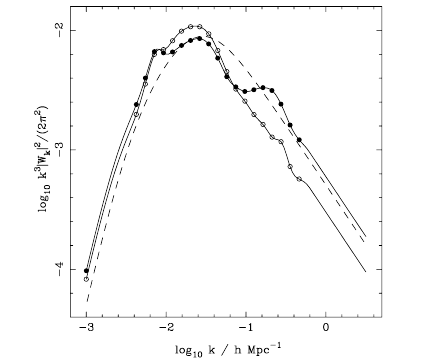
\includegraphics[width=0.4\textwidth]{../figs/2df_pk.png}	\label{fig:2df}}
	\caption{First detections of BAO}
	\label{fig:2005-results}
\end{figure}


\section{Curvature, dark matter and the expansion of the universe}
After Hubble discovered the expansion of the universe through Hubble's Law\cite{Hubble1929}
\begin{align}
	v = H_0 d
	\label{eq:ley-hubble}
\end{align}
With $v$ the recession speed (the speed at which some point in space is receeding only considering the expansion of the universe), $H_0=100h$ km s$^{-1}$ Mpc$^{-1}$ Hubble's constant, $h$ a factor that parametrizes our ignorance on the true value of $H_0$ (estimated to be around $0.67$), and $d$ the distance of said point, a great deal of studies concerning the expansion of the universe started. The most relevant result of those for this report are Friedmann's equations. \\
\begin{align}
	H^2(t) := \left(\frac{\dot a}{a}\right)^2 &=  \frac{8\pi G \rho}{3} +\frac{\Lambda c^2}{3} - k \frac{c^2}{a^2}
	\label{eq:1a-friedmann}\\
	3 \frac{\ddot a}{a} &= \Lambda c^2 - 4\pi G \left( \rho + \frac{3p}{c^2} \right) 
	\label{eq:2a-friedmann}
\end{align}
In these equations we see many new parameters. $H(t)$ is a generalization of $H_0$, $H_0$ being the value of $H(t)$ at $t=t_0$ where $t_0$ is the age of the universe. $a(t)$ is the scale factor of the universe, meaning that if a certain length measurement $\Delta x$ was taken at time $t_1$, then that same measurement would be $\frac{a(t_2)}{a(t_1)}\Delta x$ at $t_2$. $G$ is the Newton's gravitational constant, $\rho$ the density of the universe (including baryonic, dark matter, radiation and neutrinos), $\Lambda$ is the cosmological constant which contains information about Dark Energy. Finally we see $k$, which is the spatial (Gaussian) curvature of the universe. This is, asymptotical curvature. \\

These equations are a result of the Friedmann–Lemaître–Robertson–Walker metric 
\begin{align}
	ds ^2 = -c^2 dt^2  + a^2(t) \left( \frac{dr^2}{1-kr^2} +r^2d\theta ^2 + r^2 \sin^2\theta d\phi^2\right) 
	\label{eq:FLRW}
\end{align}which are a direct result of solutions to Einstein's field equations of General Relativity, which will not be covered in this work. In \eqref{eq:FLRW} one sees the usual components in a flat space Minkowskian metric 
\begin{align}
	ds^2 = -c^2dt^2 + dr^2 + r^2d\theta^2 + r^2 \sin^2\theta d\phi^2
\end{align} and some new terms, $a(t)$ and $k$. $a(t)$ is the aforementioned scale factor, and $k$ a measure of the curvature of the universe. It is easier now to see that $a(t)$ is crucial in the way lengths are measured, being an overall factor in the spatial part that is homogeneues but time-dependent. Also, one can notice how having different types of universe affects differently to the metric. For example $k=0$ yields (as one would expect) a flat universe. $k>0$ corresponds to a universe with spherical geometry and $k<0$ to a universe of hyperbolical geometry. \\

If one managed to solve \eqref{eq:1a-friedmann}, the result would be $a(t)$, a description of the history of the expansion of the universe. Moreover, it is also important to notice the relationship between the expansion of the universe and the distribution of matter in the universe. \\

From \eqref{eq:1a-friedmann} we define the density parameter $\Omega_m$ as $\frac{\rho}{\rho_{\text{c}}}$, with the critical density $\rho_{\text{c}} = \frac{3H_0^2}{8\pi G}$, which represents the transition point (for a universe without cosmological constant) between an ever expanding universe with negative curvature (open universe) and a collapsing universe with positive curvature (closed universe). Similarly from the rest of the terms in the equation \eqref{eq:1a-friedmann}
\begin{align}
 \Omega_\Lambda = \frac{\Lambda c^2}{3H^2}, \Omega_k = -\frac{kc^2}{H^2a^2} 
 \label{eq:definitions}
\end{align}
$\Omega_\Lambda$ corresponds to the density of dark energy in the universe, while $\Omega_k$ is not a density \textit{per se}, but is related to the total energy content of the universe, determining its curvature.
These parameters are what define the certain cosmology we are using, and obey the cosmic sum rule 
\begin{align}
	1 = \Omega_m + \Omega_\Lambda + \Omega_k
\end{align}
Which is just a result of dividing \eqref{eq:1a-friedmann} evaluated at present time, by  $H_0^2$. \\

Historically, the concept of cosmological expansion appeared when Hubble observed that the radiation of the nearby galaxies was all shifted towards the red end of the spectrum. Of course, since the universe is expanding and the distance between two points increases with time, the wave length of a certain radiation would also be affected by this expansion. This stretching of the wave length is what is known as \textit{redshift} 
\begin{align}
	z = \frac{\lambda_{\text{o}} - \lambda_{\text{e}}}{\lambda_{\text{e}}} = \frac{\lambda_o}{\lambda_e} - 1
	\label{eq:redshift}
\end{align}
Being $\lambda_o$ the observed wavelength and $\lambda_e$ the emitted wavelength of the considered radiation. $z$ is a measure of how much the universe stretched while the radiation travelled, and it can be related to $a(t)$ through 
\begin{align}
	\frac{\lambda_o}{\lambda_e} = 1+z = \frac{a(t_o)}{a(t_e)}
\end{align}
Which means that $z$ is a temporal variable measuring the time the radiation travelled through the universe. \\

However, this redshift $z$ should not be confused with the redshift caused by the Doppler Effect of objects moving away. The processes are different in origin, since cosmological redshift does not need relative movement to shift the radiation towards red wavelengths, it is the expansion of the universe what stretches the wavelength. On the contrary, the Doppler Effect appears when pulses emmitted at regular time are emitted further away due to the movement of the wave source. \\

We thus define the comoving distance $\Delta x'$ of a measurement $\Delta x$ as 
\begin{align}
	\Delta x' =\frac{\Delta x}{a(t)}= (1+z)\Delta x
\end{align}
i.e.\ the distance one would have measured had the expansion of the universe not existed. \\

With these definitions we can define  the observables we are interested in calculating/measuring. Firstly, through \eqref{eq:1a-friedmann} we calculate $H(z)$ as  
\begin{align}
	H(z) = H_0 \sqrt{\Omega_m(1+z)^3 + \Omega_k(1+z)^2 + \Omega_\Lambda} 
\end{align}
We also define the function of $z$ $D_H(z)$ known as the Hubble distance
\begin{align}
	D_H(z)  = \frac{c}{H(z)}
	\label{eq:DH-definition}
\end{align}
Note that for $z = 0$ $D_H$ gives us an idea of the distance at which the recession speed is greater than the speed of light in the vacuum, which is a direct consequence of \eqref{eq:ley-hubble}. $D_H$ can also be used to estimate the order of magnitud of the observable universe. \\

Through the Hubble distance we define the comoving distance 
\begin{align}
	D_C(z) = \frac{c}{H_0}\int_{0}^{z} \frac{dz'}{\sqrt{\Omega_m(1+z')^3 + \Omega_k(1+z')^2 + \Omega_\Lambda} } 
\end{align}
From this expression one defines the comoving angular diameter distance for some redshift $z$
\begin{align}
	D_A(z) = \begin{cases}
		\frac{D_H}{\left( 1+z \right) \sqrt{\Omega_k} }\sinh \left[ \sqrt{\Omega_k} D_C /D_H \right]  	 &\Omega_k >0\\
		\frac{1}{1+z}D_C& \Omega_k =  0\\
		\frac{D_H}{\left( 1+z \right) \sqrt{|\Omega_k|}} \sin \left[ \sqrt{|\Omega_k|} D_C /D_H \right]  	 &\Omega_k <0
		\label{eq:DA-definition}
	\end{cases}
\end{align}
And finally, the magnitude $D_M(z) = (1+z)D_A(z)$.

\section{$\Lambda$ Cold Dark Matter model}
\label{sec:LCDM}

In the definitions in \eqref{eq:definitions} the parameters $\Omega$ were introduced. This definitions, plus the definition of the density parameter $\Omega_m$ are part of the set of parameters that form the $\Lambda$ Cold Dark Matter ($\Lambda$CDM) model. \\

This model is the simplest available way of explaining the current state of the universe, with 6 different constants. The name is derived from two of the biggest components of the universe, $\Lambda$ (the cosmological constant, related to Dark Energy) and Cold Dark Matter, which is thought to be
\begin{itemize}
	\item \textbf{Cold}: Non relativistic ($v \ll c$)
	\item \textbf{Non baryonic}: Made up of non baryonic matter i.e. anything other than protons and neutrons (and by convention, electrons).
	\item \textbf{Disipationless}: Since Dark Matter does not interact with the electromagnetic field, it can not dissipate temperature through photon emission.
	\item \textbf{Collisionless}: Dark matter particles can only interact through gravity and possibly, the weak force and so they do not collide with one another.
\end{itemize}
The information on this cold dark matter is inside $\Omega_m$, since the density $\rho$ in
\begin{align}
	\Omega_m = \frac{\rho}{\rho_c} = \frac{\rho_b + \rho_{\text{CDM}}}{\rho_c}
\end{align}
Allowing us to define two new density parameters $\Omega_b = \frac{\rho_b}{\rho_c}$ and $\Omega_c =  \frac{\rho_\text{CDM}}{\rho}$, which are part of the six free parameters that define a certain cosmology. These are $\Omega_b$, $\Omega_c$, $H_0$, the optical density of reionization $\tau_{\text{reio}}$, the amplitude of the primordial power spectrum $A_s$, the spectral index of the primordial power spectrum $n_s$. Note there is no special choice of parameters, these are just the free parameters chosen for this work. \\

In this work, an extension of the $\Lambda$CDM model is considered. Though the standard cosmological model considers a flat universe, the curvature parameter will not be fixed to $0$ and is therefore allowed to be a free parameter, adding a new degree of freedom to the standard model (not to be confused with the particle physics standard model). This model can be further extended by considering the mass of the neutrinos, the quintaessential force (dark energy)\ldots  \\

The fiducial (starting) values of these parameters that will be used in this work are
\begin{itemize}
	\item 	$\Omega_b =  0.0481 $
	\item 	$\Omega_c =  0.2604$ 
	\item $H_0 = 67.6$ km s$ ^{-1}$ Mpc$^{-1}$
	\item $\tau_{\text{reio}} = 0.09$
	\item $A_s = 2.04031526769\cdot 10^{-9}$
	\item $n_s = 0.97$
\end{itemize}
And $\Omega _k$ that will vary between $-0.2$ and 0.2.

From these free parameters, one derives some parameters. Of those, the main interest is in $\Omega_\Lambda$, $r_s$, $D_H$, and $D_A$, 
\begin{itemize}
	\item $r_s = 147.784 $ Mpc
	\item $D_H/r_s  = 18.7$
	\item $D_A/r_s  = 18.3$
\end{itemize}
And $\Omega_\Lambda$ will vary between $0.49$ and $0.89$.

Finally, we define two more parameters $\alpha_\parallel$ and $\alpha_\perp$. These parameters measure the distortion of the measurements in two different directions. $\alpha_\parallel$ is related to the distortion parallel to the line of sight, and  $\alpha_\perp$, perpendicular to the line of sight. They are defined by 
\begin{align}
	\alpha_\parallel = \frac{\left[ D_H(z) /r_s \right] }{\left[ D_H(z)/r_s \right]^{\text{fid}} }, \, \alpha_\perp = \frac{\left[ D_A(z) /r_s \right] }{\left[ D_A(z)/r_s \right]^{\text{fid}} }
	\label{eq:alphas-def}
\end{align}
$z$ being the redshift at which the measurements were taken.
       % Añadir los diferentes capítulos con el mismo formato que tiene
%                           el fichero capitulo1.tex)
%\include{capitulo2} 
% .......
\include{resultados}

\chapter{Conclusiones}

En relación a los objetivos establecidos en el capítulo~\ref{cha:objectives}, y considerando los resultados obtenidos en el capítulo~\ref{cha:results}, se pueden extraer las siguientes conclusiones de este trabajo:

\begin{enumerate}
\item Hemos revisado e implementado la metodología de Oscilaciones Acústicas de Bariones (BAO, por sus siglas en inglés) para medir distancias cosmológicas en el Universo, y la hemos aplicado a una muestra de galaxias del Extended Baryon Oscillation Spectroscopic Survey (eBOSS).
\item Hemos utilizado software de cosmología avanzada como CLASS, RUSTICO y BRASS para desarrollar un pipeline que obtiene mediciones de distancia cosmológica de un catálogo de galaxias utilizando la técnica BAO.
\item Además, hemos desarrollado código utilizando la librería Matplotlib escrita en Python para generar visualizaciones de alta calidad de nuestros resultados.
\item Los ordenadores de alto rendimiento del grupo de investigación FQM-378 de la Universidad de Córdoba se han utilizado para calcular la Transformada Rápida de Fourier de la función de correlación de 2 puntos de las galaxias de eBOSS, y para determinar las posiciones de las características de BAO en el espectro de potencia, junto con sus incertidumbres.
\item Suponiendo un modelo cosmológico plano, nuestras mediciones de distancia inferidas a las galaxias de eBOSS (normalizadas a la escala del horizonte de sonido) son: $D_H/r_d = 18.66 \pm 0.72$ y $D_M/r_d = 18.28 \pm 0.53$ para la distancia angular, consistentes con trabajos previos.
\item Nuestro resultado principal es que no hay dependencia significativa de estas observables con respecto a cambios en el valor asumido del parámetro $ \Omega_k$ en el rango de estudio.
\end{enumerate}

Por lo tanto, concluimos que la suposición de un valor particular de $\Omega_k$ en la conversión de corrimiento al rojo a distancia no tiene ningún efecto significativo (al menos en el rango $\Omega_k \in [-0.20, +0.20]$) en las distancias cosmológicas inferidas a las galaxias de eBOSS utilizando la metodología BAO.

\setcounter{chapter}{4}
\chapter{Conclusions}

Relative to the objectives stated in the chapter~\ref{cha:objectives}, and seeing the results obtained in the chapter~\ref{cha:results}, the following conclusions can be made from this work.

\begin{enumerate}
	\item We have reviewed and implemented the Baryon Acoustic Oscillation (BAO) methodology to measure cosmological distances in the Universe, and we have applied it to a sample of galaxies from the extended Baryon Oscillation Spectroscopic Survey (eBOSS)
	\item We have used advanced cosmology software such as CLASS, RUSTICO and BRASS to develop a pipeline that obtains cosmological distance measurements of a galaxy catalogue using the BAO technique.
	\item In addition, we have developed code using the Matplotlib library written in Python to generate quality level visualization of our results.
	\item The high performance computers of the University of Cordoba FQM-378 research group have been used to calculate the Fast Fourier Transform of the 2-point correlation function of eBOSS galaxies, and to determine the positions of the BAO features in the power spectrum, together with their uncertainties.
	\item Assuming a flat cosmological model, our inferred distance measurements to eBOSS galaxies (normalized to the sound horizon scale) are: $D_H/r_d = 18.66 \pm 0.72$ and $D_M/r_d = 18.28 \pm 0.53$ for the angular diameter distance, consistent with previous works.
	\item Our main result is that there is no significant dependence of these observables with respect to changes in the assumed value of the $\Omega_k$ parameter in the range of study.
\end{enumerate}

Therefore, we conclude that the assumption of a particular $\Omega_k$ value in the redshift-to-distance conversion does not have any significant effect (at least in the range $\Omega_k \in [-0,20, +0,20]$) on the inferred cosmological distances to eBOSS galaxies using the BAO methodology.

       % Conclusiones (insertar en el fichero conclusion.tex proporcionado,
%                                          las conclusiones en español e inglés)
 
%%%%%%%%%%%%%%%%%%%%%%%%%%%%%%%%%%%%%%%%%%%%%%%%%%%%%%%%%%
%%%%  LA BIBLIOGRAFÍA %%%%%%%%%%%%%%%%%%%%%%%
%%%%%%%%%%%%%%%%%%%%%%%%%%%%%%%%%%%%%%%%%%%%%%%%%%%%%%%%%

\addcontentsline{toc}{chapter}{Bibliografía}
\begin{thebibliography}{999}
	\bibitem{Planck2018} Planck Collaboration. (2018). Planck 2018 results. VI\@. Cosmological parameters. \textit{Astronomy \& Astrophysics}, 641, A6. \url{https://doi.org/10.1051/0004-6361/201833910}

	\bibitem{Penzias1965} Penzias, A. A., \& Wilson, R. W. (1965). A Measurement of Excess Antenna Temperature at 4080 Mc/s. \textit{The Astrophysical Journal}, 142, 419. \url{https://doi.org/10.1086/148307}

\bibitem{SmootMather} Smoot, G. F., \& Mather, J. C. (1992). Structure in the COBE differential microwave radiometer first-year maps. \textit{The Astrophysical Journal}, 396, L1-L5. \url{https://doi.org/10.1086/186504}

\bibitem{2dFCole2005} Cole, S., et al. (The 2dFGRS Collaboration) (2005). The 2dF Galaxy Redshift Survey: power-spectrum analysis of the final dataset and cosmological implications. \textit{Monthly Notices of the Royal Astronomical Society}, 362, 505-534. \url{https://doi.org/10.1111/j.1365-2966.2005.09318.x}

\bibitem{Eisenstein2005} Eisenstein, D. J., et al. (The SDSS Collaboration) (2005). Detection of the Baryon Acoustic Peak in the Large-Scale Correlation Function of SDSS Luminous Red Galaxies. \textit{The Astrophysical Journal, 633, 560-574}. \url{https://doi.org/10.1086/466512}

\bibitem{Hubble1929} Hubble, E. (1929). A relation between distance and radial velocity among extra-galactic nebulae. \textit{Proceedings of the National Academy of Sciences}, 15(3), 168-173. \url{https://doi.org/10.1073/pnas.15.3.168}

\bibitem{class} Lesgourgues, J., Tram, T., \& Sprenger, T. The Cosmic Linear Anisotropy Solving System (CLASS) IV: efficient implementation of the Cosmic Microwave Background and large scale structure likelihoods. \textit{Journal of Cosmology and Astroparticle Physics}, 2011(07), 002. \url{https://github.com/lesgourg/class_public}.

\bibitem{montepython} Brinckmann, T. Montepython: Pythonic MCMC for Cosmology. \textit{Journal of Open Source Software}, 3(24), 676, 2018. \url{https://github.com/montepython/montepython_public}.

\bibitem{rustico} Gil-Marín, H. RUSTICO: A fast and scalable method for measuring the autocorrelation function of galaxy surveys. \textit{Astronomy and Computing}, 31, 100391, 2020. \url{https://github.com/hectorgil/rustico}.

\bibitem{brass} Gil-Marín, H. BRASS: BAO and RSD Analysis of Spectra with Systematics. \textit{Journal of Open Source Software}, 4(45), 1884, 2019. \url{https://github.com/hectorgil/Brass}.
\bibitem{Gil_Mar_n_2020}
Héctor Gil-Marín, et al.
\newblock The Completed {SDSS}-{IV} extended Baryon Oscillation Spectroscopic Survey: measurement of the {BAO} and growth rate of structure of the luminous red galaxy sample from the anisotropic power spectrum between redshifts 0.6 and 1.0.
\newblock \emph{Monthly Notices of the Royal Astronomical Society}, 498(2):2492--2531, Aug. 2020.
\newblock URL: \url{https://arxiv.org/abs/2007.08994}



\bibitem{eBoss}
S.~Alam \textit{et al.} [eBOSS],
%``Completed SDSS-IV extended Baryon Oscillation Spectroscopic Survey: Cosmological implications from two decades of spectroscopic surveys at the Apache Point Observatory,''
Phys. Rev. D \textbf{103}, no.8, 083533 (2021)
doi:10.1103/PhysRevD.103.083533
[arXiv:2007.08991 [astro-ph.CO]].
%588 citations counted in INSPIRE as of 19 Apr 2023

\end{thebibliography}
     % Bibliografía (insertar en el fichero bibliografia.tex proporcionado, 
%                                          la bibliografia con bibitem)

%----------------------------------------------------------
% Si se tiene una base de datos bibliográfica
% estilo de bibliografía: plana, alfa...
\nocite{*}
%
%% Bibliografía---------------------------
%% Añade la bibliografía al índice
%
%%se incluye la bibliografía. Archivo de tipo .bib (bibtex)
\bibliography{bib/jabref}
\bibliographystyle{plain}
%----------------------------------------------------------

% Apéndices (si los hubiera)
\appendix
\chapter*{Anexo: Ejemplo para introducir código Matlab}
\addcontentsline{toc}{chapter}{Anexo: Ejemplo para introducir código Matlab}

\renewcommand{\baselinestretch}{1}
\begin{lstlisting}[language=Matlab]
%% 3-D Plots
% Three-dimensional plots typically display a surface 
% defined by a function in two variables, z = f(x,y) .
%%
% To evaluate z, first create a set of (x,y) points 
% over the domain of the function using meshgrid.
	[X,Y] = meshgrid(-2:.2:2);                                
	Z = X .* exp(-X.^2 - Y.^2);
%%
% Then, create a surface plot.
	surf(X,Y,Z)
%%
% Both the surf function and its companion mesh display 
% surfaces in three dimensions. surf displays both the 
% connecting lines and the faces of the surface in color. 
% Mesh produces wireframe surfaces that color only the 
%lines connecting the defining points.

\end{lstlisting}
\renewcommand{\baselinestretch}{1.5}



    % Añadir los diferentes anexos, si los hubiera, con el mismo formato que tiene
%                     el fichero anexo1.tex)
\chapter*{Anexo: Ejemplo para introducir código ISE}

\addcontentsline{toc}{chapter}{Anexo: Ejemplo para introducir código ISE}

\lstdefinelanguage{ISE} {morekeywords={library,use,entity,is,port,in,out,end,
               architecture,of,is,signal,begin,process,then,
               port,downto,if,and,then,else
               },                
sensitive=false,
emph={STD_LOGIC_1164,
STD_LOGIC_ARITH,
STD_LOGIC_UNSIGNED,
IEEE,
ALL,
STD_LOGIC,
STD_LOGIC_VECTOR}, 
emphstyle=\color{magenta},
morecomment=[l]{--},
basicstyle=\small \ttfamily,
   keywordstyle=\color{blue},
   commentstyle=\color{webgreen},
   stringstyle=\color{webtinto},
   numbers=left,
   numberstyle=\tiny\color{gray},
   stepnumber=1,
   numbersep=10pt,
   backgroundcolor=\color{white},
   tabsize=4,
   showspaces=false,
   showstringspaces=false,
%
   frame=LtbR,
     framerule=0.5pt,
     aboveskip=0.5cm,
     framextopmargin=3pt,
     framexbottommargin=3pt,
%     framexleftmargin=1cm,
     framesep=0pt,
     rulesep=.4pt,
     backgroundcolor=\color{gray96},
     rulesepcolor=\color{black}
     }


\renewcommand{\baselinestretch}{1}
 \begin{lstlisting}[language=ISE]
library IEEE;
             use IEEE.STD_LOGIC_1164.ALL;
             use IEEE.STD_LOGIC_ARITH.ALL;
             use IEEE.STD_LOGIC_UNSIGNED.ALL;
-- Uncomment the following library declaration if 
-- instantiating  any Xilinx primitive in this code.
-- library UNISIM;
-- use UNISIM.VComponents.all;
     
entity counter is
	Port ( CLOCK : in  STD_LOGIC;
   	DIRECTION :    in  STD_LOGIC;
  	COUNT_OUT :    out STD_LOGIC_VECTOR (3 downto 0));
end counter;

architecture Behavioral of counter is
signal count_int : std_logic_vector(3 downto 0) := "0000"; 
begin
process (CLOCK)
begin
	if CLOCK='1' and CLOCK'event then
		if DIRECTION='1' then
			count_int <= count_int + 1;
		else
			count_int <= count_int - 1;
		end if;
	end if;
end process;
COUNT_OUT <= count_int;
end Behavioral;
\end{lstlisting}
\renewcommand{\baselinestretch}{1.5}



% Termina el documento
\end{document}
